\documentclass{standalone}
\usepackage{graphicx}	
\usepackage{amssymb, amsmath, amsthm}
\usepackage{color}

\usepackage{tikz}
\usetikzlibrary{intersections, backgrounds}

\definecolor{light}{RGB}{220, 188, 188}
\definecolor{mid}{RGB}{185, 124, 124}
\definecolor{dark}{RGB}{143, 39, 39}
\definecolor{highlight}{RGB}{180, 31, 180}
\definecolor{gray10}{gray}{0.1}
\definecolor{gray20}{gray}{0.2}
\definecolor{gray30}{gray}{0.3}
\definecolor{gray40}{gray}{0.4}
\definecolor{gray60}{gray}{0.6}
\definecolor{gray70}{gray}{0.7}
\definecolor{gray80}{gray}{0.8}
\definecolor{gray90}{gray}{0.9}
\definecolor{gray60}{gray}{0.95}

\begin{document}

\begin{tikzpicture}[scale=0.3]
  \begin{scope}[shift={(0, 0)}]
    \draw[white] (-17, -12) rectangle (17, 12);

    \begin{scope}
      \clip (-13, -8) rectangle (13, 8);
      \node at (0, 0) {\includegraphics[width=7.8cm]{realizations.eps}};
    \end{scope}
  
    \draw [->, >=stealth, line width=1] (-13, -8) -- +(26, 0);
    \draw [->, >=stealth, line width=1] (-13, -8.058) -- +(0, 16);
    \node[] at (0, -10) { $x$ };
    \node[] at (-15, 0) { $f(x)$ };
  \end{scope}
  
  \begin{scope}[shift={(34, 0)}]
    \draw[white] (-17, -12) rectangle (17, 12);

    \begin{scope}
      \clip (-13, -8) rectangle (13, 8);
      \node at (0, 0) {\includegraphics[width=7.8cm]{ribbons.eps}};
    \end{scope}
  
    \draw [->, >=stealth, line width=1] (-13, -8) -- +(26, 0);
    \draw [->, >=stealth, line width=1] (-13, -8.058) -- +(0, 16);
    \node[] at (0, -10) { $x$ };
    \node[] at (-15, 0) { $f(x)$ };
  \end{scope}
 
\end{tikzpicture}

\end{document}  